In this section we provide details about ESMACS and TIES specifications and
about adaptive methodologies using TIES\@. We conclude with a description and
validation of the physical systems used in this work.

% Science drivers
% -------------------------------------------------------------- Everything
% related to the chemistry/drug discovery science in this paper. ----

% In its simplest form, the aim of a drug discovery campaign is to optimize
% the efficacy of a drug molecule to a \emph{certain} target (usually a
% protein) as a function of the drug molecule itself. In the \emph{hit to
% lead}, and \emph{lead optimization} stages of the pipeline this is done by
% maximizing a quantity called the binding affinity (which is a good proxy
% for efficacy of the medication). To find the maximum binding affinity
% fidelity we have to probe large number of candidate drug molecules and find
% the best ones. The basic use case for HTBAC is to enable this type of large
% scale binding free energy studies of protein-ligand complexes using
% ensemble simulations.

% Given the very large number of drug candidates, it is imperative to gain
% maximum insight into potential candidate compounds using time and resources
% efficiently. This provides one clear motivation for the use of adaptive
% methods which minimize the compute time used whilst producing binding free
% energy estimates meeting pre-defined quality criteria (such as convergence
% or statistical uncertainty below a given threshold).

% Both ESMACS and 
% TIES have been successfully used to predict binding affinities quickly and 
% accurately~\cite{Wan2017brd4, Bhati2017}.

% ---------------------------------------------------------------------------
\subsection{ESMACS and TIES}\label{ssec:esm_ties}

ESMACS and TIES~\cite{Wan2017brd4, Bhati2017} are two free energy calculation
protocols that implement absolute and relative methods, respectively.
Absolute free energy methods calculate the binding affinity of a
\emph{single} drug molecule to a protein, while relative methods calculate
the \emph{difference} in binding affinity between two (usually similar in
structure) drug molecules. 
Both protocols are designed to use an ensemble MD simulation approach to enhance the reproducibility and accuracy of standard free energy calculation techniques 
(MMPBSA~\cite{Massova1999} in the case of ESMACS and thermodynamic 
integration~\cite{Straatsma1988, Straatsma1991} in TIES).
The use of ensemble averaging allows tight control of error bounds in the 
resulting free energy estimates.

ESMACS and TIES consists of three main steps: minimization, equilibration and
production MD (in its current implementation all MD steps are conducted in 
NAMD~\cite{Phillips2005}). In practice, the equilibration phase is broken into 
multiple steps to ensure that the size of the simulation box does not alter too 
much over the simulation. During these steps, positional constraints are 
gradually released from the structure and the physical system is heated to a
physiologically realistic temperature.

Whilst both protocols share a common sequence of steps, the make-up of the
ensemble is different. In ESMACS, an ensemble consists of a set of 25
\textbf{replicas}, i.e., identical simulations differing only in the initial
velocities assigned to each atom. In TIES, the ensemble contains a set of
\textbf{$\lambda$} windows, each spawning a set of replicas. As a
transformation parameter $\lambda$ increases from 0 to 1, the system
description transforms from containing an initial drug to a target compound
via a series of hybrid states. Sampling along $\lambda$ is then required to
compute the difference in binding free energy. In previous studies, TIES has
been deployed using 65 replicas, evenly distributed among 13 $\lambda$
windows. Following the completion of the simulation steps, both protocols
require the execution of free energy analysis steps. The detailed composition
of ESMACS and TIES protocols is shown in Fig.~\ref{fig:ties_esmacs_application}.

\begin{figure}
  \centering
  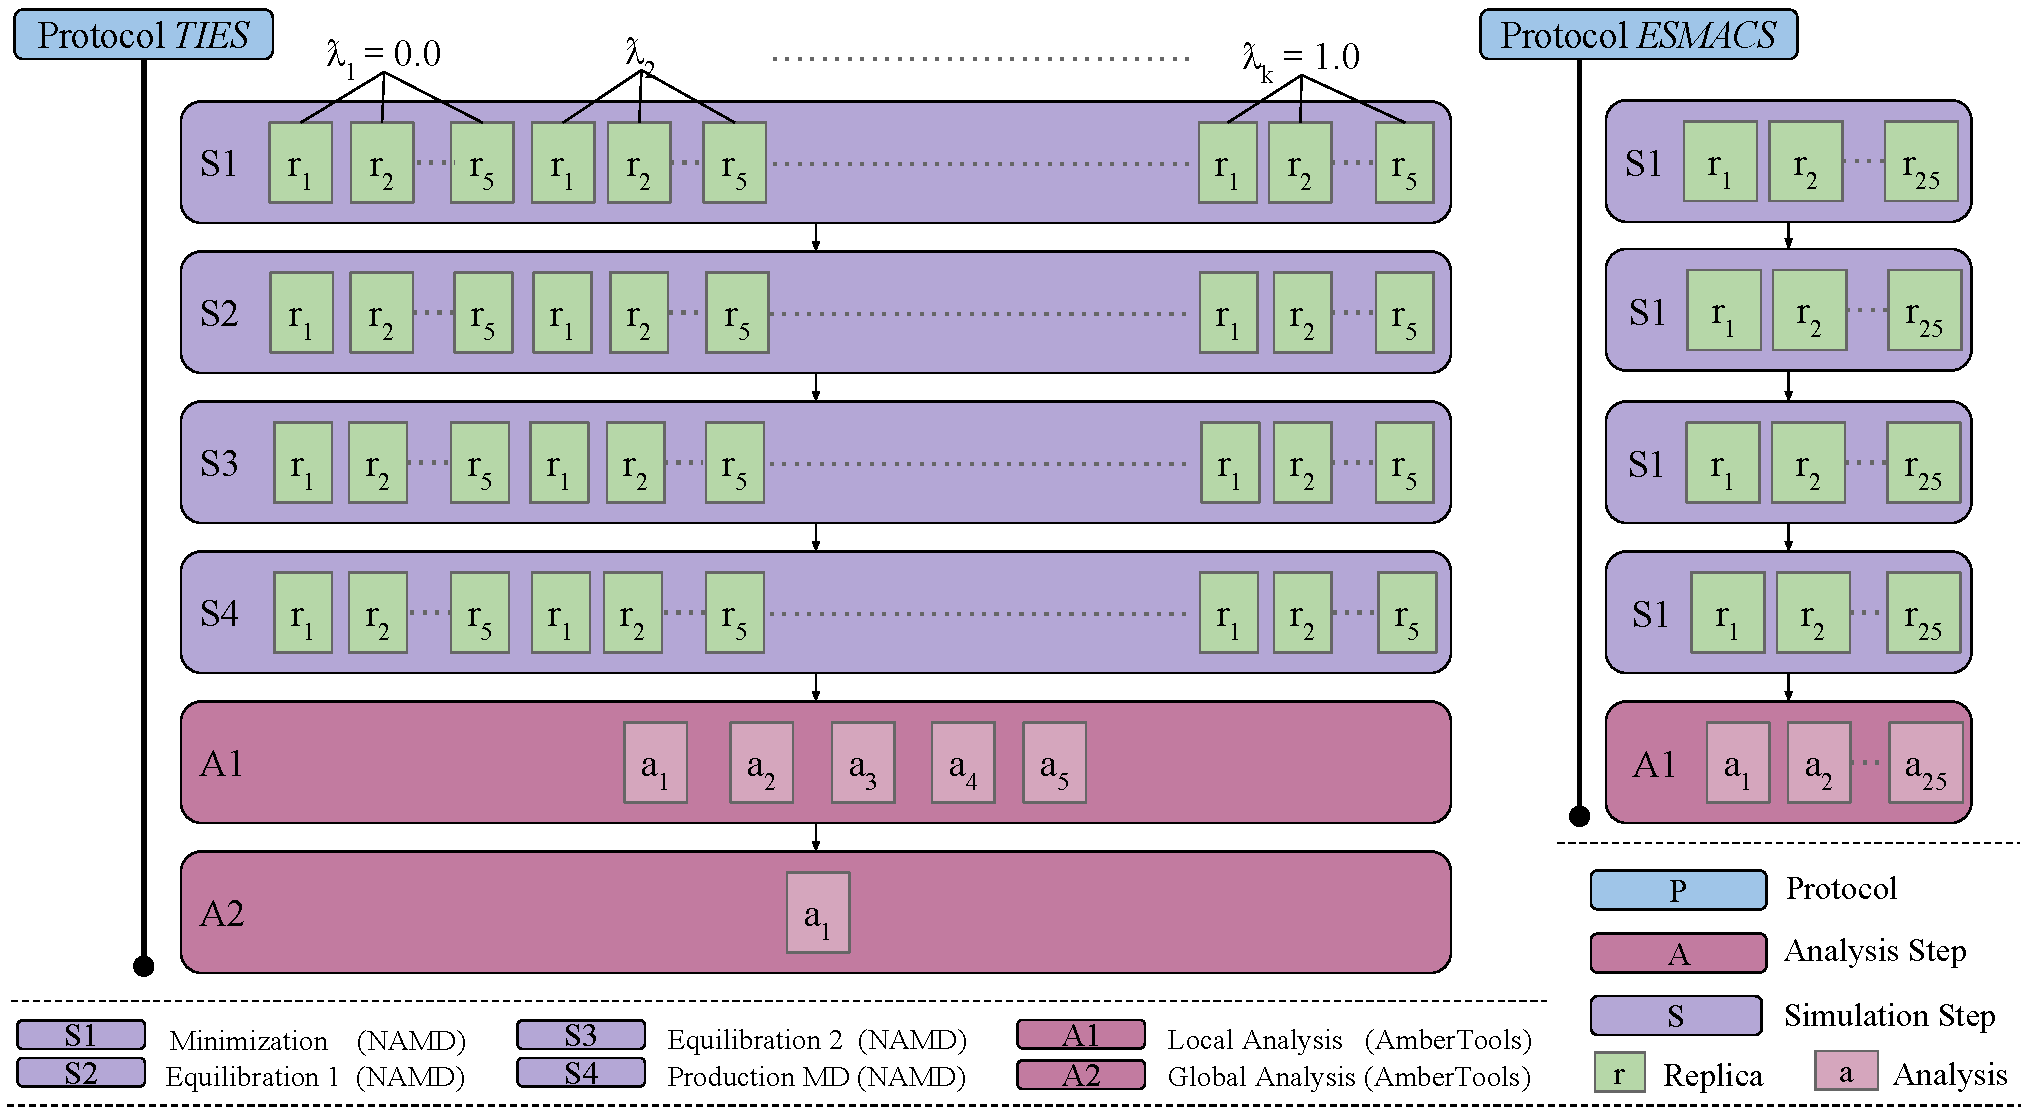
\includegraphics[width=\columnwidth]{figures/ties_esmacs_application_model.pdf}
  \caption{TIES and ESMACS protocols consist of simulations steps followed by
  analysis step(s). ESMACS contains 25 replicas per simulation step; TIES
  contains 5 replicas per $\lambda$ window. We model TIES with 13 $\lambda$
  windows, spawning 65 replicas in each simulation step. All replicas
  simulate 6ns.}\label{fig:ties_esmacs_application}
\up{}
\up{}
\end{figure}

% The drug discovery pipeline is continuously evolving and morphing from a
% fully experimental procedure, to stages of it being replaced by
% computational methods, like computer aided drug design.

% Intro to binding affinity
% ----------------------------------------------------

% There exists two types of free energy calculation protocols: absolute and
% relative. Absolute free energy methods calculate the binding affinity of a
% \emph{single} drug molecule to a protein, while relative methods calculate
% the \emph{difference} in binding affinity between two (usually similar in
% structure) drug molecules. The computational requirements of the two
% protocols differ sometimes significantly, but deciding which one is more
% appropriate for the task at hand is not trivial, as it is a function of
% resources, required time to convergence, accuracy thresholds etc.

% Using these protocols, we have demonstrated the lack of reproducibility of
% binding affinities derived from individual simulations for a variety of
% protein systems, with calculations for the same protein-ligand combination
% (using almost identical initial conditions) producing results varying by up
% to 12 kcal mol $^{-1}$ for small molecules, whilst flexible ligands can
% vary even more~\cite{Sadiq2010, Wright2014}.

% TIES is a so called ``alchemical'' relative free energy method in which the
% fact that the potential used to describe the system is user definable to
% transform one system into another. This allows for the calculation of free
% energy differences between the two systems, such as those induced by an
% alteration to a candidate drug.

% The computational requirements of the two protocols differ sometimes
% significantly, but deciding which one is more appropriate for the task at
% hand is not trivial, as it is a function of resources, required time to
% convergence, accuracy thresholds etc. TIES is based on rigorous, but
% computationally expensive, calculations of relative free energies. ESMACS,
% in contrast, provides absolute binding free energies at low computational
% cost, but to achieve this coarse grains many of the details of the physical
% system being studied.

% In order to obtain a meaningful TIES result it is necessary to not only
% simulate the drug pair in the protein but also in an aqueous environment,
% adding a further 65 replicas albeit it using a smaller system at lower
% computational cost.

% Both protocols are highly customizable, for example the number of
% simulation replicas in the ensemble and the lengths of their runs can be
% varied.

% All replicas within a simulation step are assigned simulation timesteps
% based \jdnote{UCL please provide the end of sentence $S1=1000$;
% $S2=30,000$; $S3=800,000$; $S4=2,000,000$.}

% In addition, the ESMACS protocol can also be extended to account for
% adaptation energies involved in altering the conformation of the protein or
% ligand during binding through the use of separate component simulations.


% Some notes on ensembles and replicas.
% ----------------------------------------

%In addition, the ability to run replica simulations concurrently means that,
%as long as sufficient compute resources are available, turnaround times can
%be significantly reduced compared to the generation of single long
%trajectories. Due to their shared philosophical underpinning both protocols
%share similar middleware requirements.

% Indeed, our work has revealed how completely unreliable single simulation
% based approaches are. We have shown that averaging across multiple runs
% reliably produces results in agreement with previously published
% experimental findings~\cite{Sadiq2010, Wan2011, Wright2014, Bhati2017,
% Wan2017brd4, Wan2017trk}, and correctly predicted the results of
% experimental studies performed by colleagues in
% collaboration~\cite{Bunney2015}. We term this approach ensemble molecular
% dynamics, ``ensemble'' here referring to the set of individual (replica)
% simulations conducted for the same physical system.

% First a quick intro to NAMD, then generic simulation protocol description.
% ---

% The current implementation of both TIES and ESMACS uses the the NAMD
% package~\cite{Phillips2005} to conduct the simulations.

% TIES and ESMACS intro
% --------------------------------------------------------

%  Upon completion of the MD simulation, free energy computations are
% performed on a per replica basis and then globally across all ensembles.

%~\cite{amber14, Case2005, MillerIII2012}.

% TIES more details
% ------------------------------------------------------------

% Analysis
% ---------------------------------------------------------------------
%---------------------------------------------------------------------------
%
% move this section to fe_protocols.tex

% Adaptive quadrature is a numerical integration algorithm that is designed
% to minimize the number of function evaluations while still achieving a
% given error tolerance when estimating the integral. We use this algorithm
% to minimize the number of full simulations that are required to be run,
% while still keeping the high accuracy of the protocol.

% ---------------------------------------------------------------------------
\subsection{The Value of Adaptivity}\label{ssec:adapt_ties}

The main driver for adaptivity is that computational campaigns will typically
involve compounds with a wide range of chemical properties which can impact
the time to convergence and the type of sampling required to gain accurate 
results. There may be cases where it is important to increase the sampling of 
phase space, possibly through expanding the ensemble. In general, there is no 
way to know exactly which calculation setup a particular system requires before 
runtime.

Another driver of adaptivity is that, on occasion, alchemical methods may
converge very slowly. 
% In such circumstances, use of another method, such as ESMACS, may be the
% best option.
This means that the most effective way to gain accurate and precise free
energy results on industrially or clinically relevant timescales is 
% to be able 
to adapt both sampling (\textbf{intra-protocol}) and the type of calculation
(\textbf{inter-protocol}) used at runtime. With potentially thousands of
simulations, often employing multiple analysis methodologies, this provides
the most effective way to utilize these techniques and resources at scale.

In TIES, the change in free energy associated with the transformation is
calculated using an adaptive quadrature function which numerically integrates
the values of the $\partial U/\partial\lambda$ across the full set of
simulated $\lambda$ windows. Obtaining accurate and precise results from TIES
using adaptive quadratures requires that the $\lambda$ windows correctly
capture the changes of $\partial U/\partial\lambda$ over the transformation.
This behavior is highly sensitive to the chemical details of the compounds
being studied and varies considerably among candidates. Typically,
$\lambda$ windows are evenly spaced between 0 and 1 with the spacing between
them set before execution at a distance determined by the simulator to be
sufficient for a wide range of systems.

However, the number or the location of the $\lambda$ windows that will most
impact the calculation are not known \textit{a priori}, and varies across
candidates. As each window requires multiple simulations, sampling
with a high frequency is expensive. % and impractical. 
Approximations using evenly spaced $\lambda$ windows reach an acceptable
accuracy threshold but adaptive placement of $\lambda$ windows is likely to
better capture the shape of the $\partial U/\partial\lambda$ curve, leading
to more accurate and precise results for a comparable computational cost.

In this work, we use adaptive middleware to automate runtime decisions based
on partial simulation data, and redistribute resources at runtime
to support dynamically generated simulations. We focus on 
% one type of adaptivity, 
intra-protocol adaptivity which relies on
intermediate runtime results
\textit{within} a protocol instance to define the % next 
following set of % further
simulations. % requirements. 
% In TIES, the optimal positions of the $\lambda$
% windows are not known \textit{a priori}. Therefore, the number of simulations
% and their descriptions, which are dictated by the $\lambda$ windows
% parameter, cannot be accurately specified before execution.
Instead of approximating the placement of all the $\lambda$ windows prior to
execution, we run TIES with less $\lambda$ windows and shorter bursts of
simulations, analyzing intermediate runtime results (i.e., trajectories) to
seed new and ideally placed $\lambda$ windows.

% Consequently, whereas in ESMACS replicas run simulations on samples using
% the same system description, in TIES replicas sample at different points
% along $\lambda$.

% Given the very large number of drug candidates, it is imperative to gain
% maximum insight into potential candidate compounds using time and resources
% efficiently. This provides one clear motivation for the use of adaptive
% methods which minimize the compute time used whilst producing binding free
% energy estimates meeting pre-defined quality criteria (such as convergence
% or statistical uncertainty below a given threshold).
  
% Drug discovery programmes usually have limited resources, and require a
% resource budget carefully looking to gain maximum insight into potential
% candidate compounds.

%  Nonetheless, they are very expensive computationally, and optimizing the
% execution time while still improving the accuracy is desirable.

%----------------------------------------------------------------------------
% move this section to fe_protocols.tex

% Figure~\ref{fig:adaptive_ties} shows our design of capturing adaptivity
% within TIES using an iterative pipeline of two stages: a short simulation
% step (1 nanosecond) followed by the adaptive quadrature analysis which
% determines optimal sampling positions \mtnote{is placement the correct term
% here? In the previous paragraph we wrote about number of simulations and
% their description, not about their placement}\jdnote{changed to optimal
% sampling position} of further simulations. We initially assign TIES with
% $y$ evenly-spaced $\lambda$ windows, which generates $y \times n$ initial
% replicas. After the first simulations finish executing, the adaptive
% quadratures function aggregates simulation results and determines where to
% assign new $\lambda$ windows.

% After the first simulation step, the analysis step operates on the
% simulation results to determine the next placement of $\lambda$ windows and
% to generate a second simulation step with new configurations.

% Each simulation step consists of multiple tasks that simulates 1 nanosecond
% of \ldots \mtnote{please add here what we are simulating}. The analysis
% consists of a single task that computes adaptive quadrature calculations %
% (as defined in section~\ref{sec:science-drivers}) to determine whether to
% spawn additional $\lambda$ windows \textit{in between} existing windows.
% This enables continuous execution of existing simulations and beginning of
% new simulations \mtnote{I do not understand this sentence. Can we eliminate
% it?}. The workflow is executed iteratively until the total simulation
% duration defined by the user is reached, determining termination.

% \begin{figure}
%   \centering
%   \includegraphics[width=\columnwidth]{figures/adaptive_TIES_workflow_diagr
%   am.pdf}
%   \caption{Intra-protocol adaptivity using TIES with multiple concurrent
%   and independent simulations. The analysis (adaptive quadratures) operates
%   on a snapshot of the current simulations for each $\lambda$ window, and
%   decides whether the critical accuracy threshold is reached, else current
%   simulations continue executing and additional $\lambda$ windows are
%   assigned in order to account for additionally needed simulations in
%   specific regions of the phase- space}
% \label{fig:adaptive_ties}
% \end{figure}